
%(BEGIN_QUESTION)
% Copyright 2012, Tony R. Kuphaldt, released under the Creative Commons Attribution License (v 1.0)
% This means you may do almost anything with this work of mine, so long as you give me proper credit

A model rocket enthusiast wants to approximately measure the peak altitude of her rocket by measuring the angle from horizontal ($\theta$) sighting the rocket at its apogee and the distance from the launch pad to the point of observation.  Which trigonometric function will she need to use in order to calculate the rocket's height?

$$\includegraphics[width=15.5cm]{i02680x01.eps}$$

\begin{itemize}
\item{(A)} Tangent
\vskip 5pt 
\item{(B)} Cosine
\vskip 5pt 
\item{(C)} Cosecant
\vskip 5pt 
\item{(D)} Sine
\vskip 5pt 
\item{(E)} Secant
\end{itemize}

\underbar{file i02680}
%(END_QUESTION)





%(BEGIN_ANSWER)

The ``tangent'' function is the proper one to use, since the rocket's height is the side {\it opposite} the angle and the distance between the enthusiast and the launch pad is the side {\it adjacent} to the angle.

$$\tan \theta = {\hbox{Opposite side length} \over \hbox{Adjacent side length}}$$

In this particular example, the rocket's height ($h$) may be calculated from the angle ($\theta$), the launch-pad distance ($d$) and the person's height ($x$) as such:

$$h = x + d \tan \theta$$
 
%(END_ANSWER)





%(BEGIN_NOTES)


%INDEX% Mathematics review: trigonometric calculations

%(END_NOTES)


